% Options for packages loaded elsewhere
\PassOptionsToPackage{unicode}{hyperref}
\PassOptionsToPackage{hyphens}{url}
\documentclass[
]{article}
\usepackage{xcolor}
\usepackage{amsmath,amssymb}
\setcounter{secnumdepth}{-\maxdimen} % remove section numbering
\usepackage{iftex}
\ifPDFTeX
  \usepackage[T1]{fontenc}
  \usepackage[utf8]{inputenc}
  \usepackage{textcomp} % provide euro and other symbols
\else % if luatex or xetex
  \usepackage{unicode-math} % this also loads fontspec
  \defaultfontfeatures{Scale=MatchLowercase}
  \defaultfontfeatures[\rmfamily]{Ligatures=TeX,Scale=1}
\fi
\usepackage{lmodern}
\ifPDFTeX\else
  % xetex/luatex font selection
\fi
% Use upquote if available, for straight quotes in verbatim environments
\IfFileExists{upquote.sty}{\usepackage{upquote}}{}
\IfFileExists{microtype.sty}{% use microtype if available
  \usepackage[]{microtype}
  \UseMicrotypeSet[protrusion]{basicmath} % disable protrusion for tt fonts
}{}
\makeatletter
\@ifundefined{KOMAClassName}{% if non-KOMA class
  \IfFileExists{parskip.sty}{%
    \usepackage{parskip}
  }{% else
    \setlength{\parindent}{0pt}
    \setlength{\parskip}{6pt plus 2pt minus 1pt}}
}{% if KOMA class
  \KOMAoptions{parskip=half}}
\makeatother
\usepackage{longtable,booktabs,array}
\usepackage{caption}
\captionsetup[table]{skip=6pt}
\newcounter{none} % for unnumbered tables
\usepackage{calc} % for calculating minipage widths
% Correct order of tables after \paragraph or \subparagraph
\usepackage{etoolbox}
\makeatletter
\patchcmd\longtable{\par}{\if@noskipsec\mbox{}\fi\par}{}{}
\makeatother
\usepackage{graphicx}
\makeatletter
\newsavebox\pandoc@box
\newcommand*\pandocbounded[1]{% scales image to fit in text height/width
  \sbox\pandoc@box{#1}%
  \Gscale@div\@tempa{\textheight}{\dimexpr\ht\pandoc@box+\dp\pandoc@box\relax}%
  \Gscale@div\@tempb{\linewidth}{\wd\pandoc@box}%
  \ifdim\@tempb\p@<\@tempa\p@\let\@tempa\@tempb\fi% select the smaller of both
  \ifdim\@tempa\p@<\p@\scalebox{\@tempa}{\usebox\pandoc@box}%
  \else\usebox{\pandoc@box}%
  \fi%
}
% Set default figure placement to htbp
\def\fps@figure{htbp}
\makeatother
\setlength{\emergencystretch}{3em} % prevent overfull lines
\providecommand{\tightlist}{%
  \setlength{\itemsep}{0pt}\setlength{\parskip}{0pt}}
\usepackage[]{biblatex}
\addbibresource{refs.bib}
\usepackage{bookmark}
\IfFileExists{xurl.sty}{\usepackage{xurl}}{} % add URL line breaks if available
\urlstyle{same}
% fallback for those not using the hyperref driver hyperxmp:
\makeatletter
\@ifundefined{xmpquote}{\newcommand{\xmpquote}[1]{#1}}{}
\makeatother
\hypersetup{
  pdftitle={Remembering What the Map Cannot See: Contact Memory for Indoor Drone Navigation Among Unmapped Obstacles},
  pdfauthor={Abhinav Kumar (affiliation TBD)},
  hidelinks,
  pdfcreator={LaTeX via pandoc}}

\title{Remembering What the Map Cannot See: Contact Memory for Indoor
Drone Navigation Among Unmapped Obstacles}
\usepackage{etoolbox}
\makeatletter
\providecommand{\subtitle}[1]{% add subtitle to \maketitle
  \apptocmd{\@title}{\par {\large #1 \par}}{}{}
}
\makeatother
\subtitle{FIRST DRAFT --- not for circulation}
\author{Abhinav Kumar (affiliation TBD)}
\date{Draft of 21 November 2026}

\begin{document}
\maketitle
\begin{abstract}
Indoor drones plan on maps built from depth cameras, and those maps miss
exactly the obstacles that are most dangerous indoors: glass, thin
railings, netting and posts that the sensor loses. We started from
AHPPA, an adaptive planner portfolio that switches between grid A*, Lazy
Theta* and a clearance-aware A* according to the free space around the
drone, and we evaluated it honestly. On 1,320 planning queries over 44
layouts the switching rule did not pay off: always running Lazy Theta*
gave shorter paths than the portfolio, and a simple line-of-sight
smoothing of the A* path matched Lazy Theta* to within 0.2 \% at 2 \% of
extra planning time (AHPPA v2). In 2,200 simulated missions with an
incrementally built map, the portfolio's deadlock watchdog never fired:
on a map that eventually sees every obstacle, nothing gets stuck. Real
deadlocks come from obstacles the map never holds. We therefore propose
\textbf{contact memory} (AHPPA v3): when the drone is stopped or knocked
back by something its map says is free, a virtual barrier is written
across the direction of travel and the next plan is made in an escape
mode; barriers from several contacts that lie on one line are fused into
a single surface (v3.1), and memory that seals every route is relaxed in
steps. PX4/Gazebo flights against an invisible glass pane show that
contact is a violent bump that ended the flight on about half of all
contacts, so the quantity to minimise is the number of contacts per
mission. In simulation under this bump model, every map-based planner
bounced off unmapped obstacles 17--80 times per mission and completed 41
\% of missions; contact memory completed 100 \% with 1.6 contacts per
mission, and fusion removed 11 \% of the remaining contacts (paired
Wilcoxon p = 0.0013). In 103 valid PX4 software-in-the-loop flights
against an unseen glass pane, contact memory crashed in 61 \% of flights
against 95 \% for v2 (Fisher p = 0.003) and reached the goal in 33 \%
against 5 \% (p = 0.012); reacting to a detected contact by holding and
backing off raised the share of flights that survived their first
contact from 25 \% to 81 \% (p \textless{} 0.001). In flight, fusion
reduced re-contacts after relaxation (3.0 against 4.9, p = 0.002) but
did not improve outcomes.
\end{abstract}

\section{Introduction}\label{introduction}

Small multirotors flying indoors build an occupancy map from on-board
depth sensing and plan through it. The map is the planner's whole world:
a cell it believes free is a cell the planner will happily route
through. Indoors, the obstacles that depth cameras miss are common and
structurally similar --- glass walls and doors, balcony railings of thin
posts, safety netting --- and the map can also \emph{lose} a thin
obstacle it saw once, as we observed in an earlier flight test where an
OctoMap dropped 5 cm railing posts and the drone was pinned against them
until it flipped.

This paper reports a project that set out to improve planning quality
and ended up being about planning robustness. Its contributions are:

\begin{enumerate}
\def\labelenumi{\arabic{enumi}.}
\tightlist
\item
  \textbf{A negative result on planner switching.} We evaluate AHPPA, an
  adaptive portfolio of grid A* \autocite{hart1968astar}, Lazy Theta*
  \autocite{nash2010lazy} and a clearance-aware A*, against its own
  members on 1,320 queries in 44 indoor layouts, and in 2,200 full
  missions on incrementally sensed maps. The clearance-based switching
  rule is worse than always using the best member; a cheap
  post-processing step (line-of-sight smoothing of the A* path,
  \emph{AHPPA v2}) recovers the any-angle path length at the cost of
  grid A*. Its deadlock escape never fires when every obstacle is
  eventually sensed.
\item
  \textbf{Contact memory (AHPPA v3).} A planner-agnostic mechanism that
  turns a physical contact with an unmapped obstacle --- detected as a
  sudden tilt after calm flight, or as commanded-but-not-moving --- into
  a virtual barrier in every later plan, with an escape replan and a
  relaxation ladder for barriers that seal the only route.
\item
  \textbf{Surface fusion (v3.1).} Contacts are points on the unseen
  surface; barriers whose contacts lie on one line are fused into one
  segment along that line, fixing a failure seen in flight where
  barriers drawn across an oblique heading let the next route slip past
  their tips into the same pane.
\item
  \textbf{An evaluation grounded in flight data.} PX4/Gazebo flights
  show that contact is a bump, not a pin, and that each contact ends the
  flight with probability about 0.5. We build that into a simulator,
  evaluate seven planners on six unmapped-obstacle scenarios, and test
  v2, v3 and v3.1 in 110 PX4 software-in-the-loop flights (103 valid).
\end{enumerate}

\section{Related work}\label{related-work}

\textbf{Grid and any-angle planning.} A* \autocite{hart1968astar} on an
8-connected grid produces paths restricted to 45° headings; Theta*
\autocite{nash2007theta} and Lazy Theta* \autocite{nash2010lazy} relax
this with line-of-sight checks, and D* Lite
\autocite{koenig2002dstarlite} repairs a plan incrementally as the map
changes. Our v2 result --- that smoothing the A* path recovers nearly
all of the any-angle saving --- is consistent with the observation that
most of the any-angle gain on indoor maps comes from long straight runs.

\textbf{Algorithm selection and portfolios.} Choosing among algorithms
per instance is the algorithm selection problem
\autocite{rice1976algorithm}; running several and taking the first or
best answer is an algorithm portfolio \autocite{gomes2001portfolios}.
Selection pays off only when no single member dominates across instances
\autocite{kerschke2019survey}. Our analysis finds that condition
violated for indoor path length: Lazy Theta* was the best member on
1,312 of 1,318 queries.

\textbf{Mapping transparent and thin obstacles.} Glass is a known blind
spot of depth and laser sensing; vision approaches detect it from
appearance \autocite{mei2020glass}, and laser approaches exploit the
angle dependence of reflections \autocite{foster2013glass}. These
reduce, but do not remove, the chance of an unmapped obstacle; contact
memory is a complementary last line of defence that needs no extra
sensor.

\textbf{Collision-tolerant flight.} Caged and gimballed airframes
survive contact by design \autocite{briod2014gimball}, and some work
maps the environment by flying into it \autocite{mulgaonkar2018tiercel}
or uses collisions as measurements \autocite{lew2019contact}. Our
setting is the opposite: a standard, uncaged airframe for which contact
is dangerous, and the planner's job is to make the \emph{first} contact
the last one.

\section{Background: the AHPPA portfolio and what the data
said}\label{background-the-ahppa-portfolio-and-what-the-data-said}

The navigator plans on a 0.1 m occupancy grid derived from an OctoMap
\autocite{hornung2013octomap}, on three altitude layers (1.2, 1.8 and
2.4 m), with a 0.4 m safety margin. The shipped AHPPA dispatcher
measured the free space around the drone and chose grid A* in open
space, Lazy Theta* in medium clutter and a clearance-weighted A* in
tight space, with a deadlock watchdog (net displacement under 0.3 m over
6 s) that forced an escape replan with the clearance planner.

\textbf{Static queries.} On 1,320 start--goal queries drawn from 44
indoor layouts (20 families, including multi-room houses, offices and
two-storey buildings), Fig. 1 and Table 1 compare the policies. Lazy
Theta* alone shortened paths by 4.0 \% relative to stock A* but took
2.8× its planning time. The shipped portfolio got 2.65 \%; fixing its
medium mode to use Lazy Theta* got 3.79 \% at 2.7× stock time. Smoothing
the stock A* path by greedily replacing waypoint chains with
line-of-sight shortcuts (AHPPA v2) got 3.80 \% at +2 \% planning time,
and was within 1 \% of Lazy Theta* on 93 \% of queries. No
clearance-based switching rule we tried, including a learned one, beat
always using the best single member.

\begin{figure}
\centering
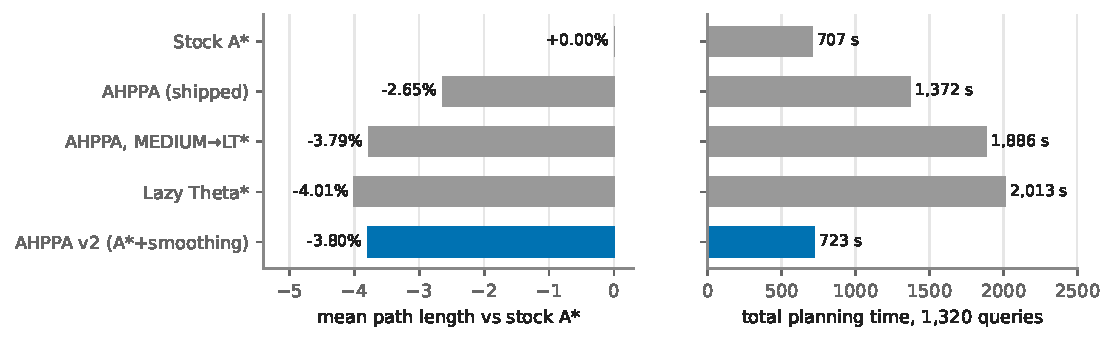
\includegraphics[width=1\linewidth,height=\textheight,keepaspectratio,alt={Fig.
1. Static planning over 1,320 queries in 44 layouts. Smoothing the grid
A* path (v2) gives nearly the any-angle path length at grid-A*
cost.}]{figs/fig_static.pdf}
\caption{Fig. 1. Static planning over 1,320 queries in 44 layouts.
Smoothing the grid A* path (v2) gives nearly the any-angle path length
at grid-A* cost.}
\end{figure}

\begin{longtable}[]{@{}lrrr@{}}
\caption{Table 1. Static planning. Minimum clearance to obstacles was
the same for all policies (0.59 m).}\tabularnewline
\toprule\noalign{}
Policy & Length vs stock & Total planning time & Solved \\
\midrule\noalign{}
\endfirsthead
\toprule\noalign{}
Policy & Length vs stock & Total planning time & Solved \\
\midrule\noalign{}
\endhead
\bottomrule\noalign{}
\endlastfoot
Stock A* & 0 \% & 707 s & 1,320 \\
AHPPA (shipped) & −2.65 \% & 1,372 s & 1,320 \\
AHPPA, medium → Lazy Theta* & −3.79 \% & 1,886 s & 1,320 \\
Lazy Theta* (no budget) & −4.01 \% & 2,013 s & 1,317 \\
\textbf{AHPPA v2 (A* + smoothing)} & \textbf{−3.80 \%} & \textbf{723 s}
& \textbf{1,320} \\
\end{longtable}

\textbf{Full missions.} We then flew 2,200 simulated missions (44
layouts × 10 missions × 5 planners) in which the drone starts with an
empty map, senses walls within 5 m (including floor and ceiling bands),
checks the path ahead after every sensor sweep and replans when it is
blocked. Mission success was 94.8 \% for stock A*, smoothed A* and v2,
94.1 \% for the shipped portfolio and 93.0 \% for Lazy Theta*; failures
were timeouts in the same few cluttered layouts for every planner, and
there were no collisions. Mission time was statistically
indistinguishable between v2 and stock A* (+0.9 \%, p = 0.91), while
Lazy Theta*'s planning hover made it 12.7 \% slower (p = 4.5 × 10⁻⁷).
\textbf{The deadlock watchdog fired zero times in 2,200 missions.} With
a map that eventually contains every obstacle, a kinematically faithful
drone always keeps moving; the escape mode, the portfolio's most
distinctive safety component, had nothing to do.

This was the turning point of the project: the failure the watchdog was
built for --- the drone pinned against railing posts in our earlier
flight test --- is caused by an obstacle the map \emph{does not hold},
and no amount of replanning on that map can route around it.

\section{Contact memory}\label{contact-memory}

\subsection{Detecting contact}\label{detecting-contact}

The navigator runs three detectors, all of which report the drone
position \(p\) and the heading \(h\) it was trying to fly:

\begin{itemize}
\tightlist
\item
  \textbf{Impact.} Tilt crosses 10° after at least 1 s of calm flight
  (tilt below 5°). In PX4 flights normal cruise stayed below 3.4° and
  contacts produced 10--43° within 0.1 s. The heading is the direction
  of motion over the calm window before the impact.
\item
  \textbf{Fast stuck.} The drone has been commanded along a path for 1.5
  s but moved less than 0.1 m (not checked near the goal or while
  hovering to plan).
\item
  \textbf{Watchdog.} The original 6 s / 0.3 m deadlock watchdog.
\end{itemize}

After an impact the navigator does not fight the bounce for 0.3 s, then
backs off 0.6 m opposite the heading at the current yaw, and waits until
the drone is steady (tilt \textless{} 5°, speed \textless{} 0.2 m/s, at
the hold altitude, for 1 s; minimum 2 s, maximum 10 s) before
replanning.

\subsection{Barriers}\label{barriers}

Each report stores a barrier centred \(d = 0.3\) m ahead of the drone,
\(c = p + d\,h\), with the heading. In planning, each barrier is drawn
as a segment of width \(W\) across the heading, inflated by the safety
margin plus 0.3 m (the position of the unseen surface is uncertain), on
every altitude layer (an obstacle that stopped the drone is assumed
floor-to-ceiling), and the next plan uses the clearance planner (escape
mode). We use a \emph{wall hypothesis}, \(W = 4\) m: the obstacles
indoor maps miss are long and straight. In simulation, stuck events per
mission were 3.41, 2.88, 2.75 and 3.18 for \(W\) = 1.2, 2, 4 and 8 m; 8
m sealed real passages.

\subsection{Surface fusion (v3.1)}\label{surface-fusion-v3.1}

A barrier across the heading is aligned with the surface only for a
head-on contact. In PX4 flights the drone hit a flat pane at up to 33°
from its normal; the barrier was tilted against the pane, and the
replanned route passed its tip and hit the same pane again (Fig. 2,
left). Contact points, however, \emph{are} samples of the surface. v3.1
groups barriers greedily: a barrier joins a group if its centre is
within 5 m of a member, all centres lie within 0.4 m of their principal
line, every heading points into that line (\(|h\cdot u| \le 0.8\) for
line direction \(u\)), and the headings agree with each other
(\(h_i\cdot h_j \ge 0.5\), so that contacts on the two faces of an
L-shaped corner are not merged). A group becomes one segment along its
principal line, spanning the contacts' projections plus \(W/2\) at each
end.

\subsection{Relaxation ladder}\label{relaxation-ladder}

A barrier can seal the only route --- an unseen post in the middle of
the only doorway. If no path exists, v3 retried with each barrier
reduced to its contact point, then without memory. In flight, this dot
fallback sent the drone back into a pane it had already hit twice. v3.1
inserts a level between them, the \emph{hull}: each group's measured
span plus 0.5 m at each end, which is surface the drone has actually
touched. The ladder is bar → hull → dot → none, and it restarts at
``bar'' for every plan.

\begin{figure}
\centering
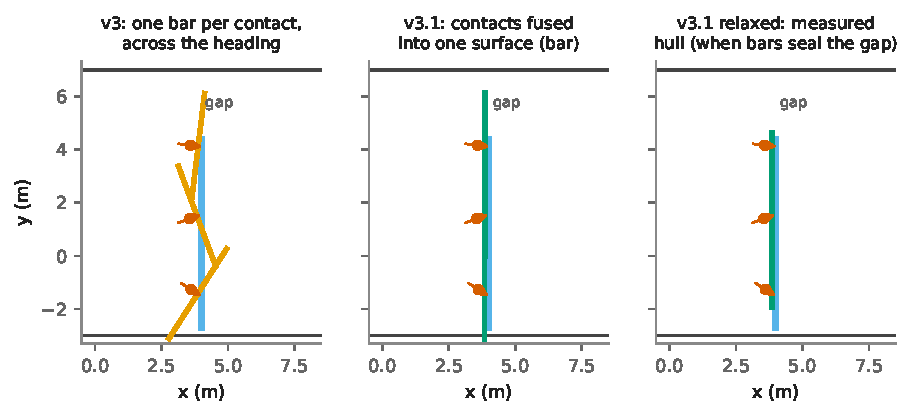
\includegraphics[width=1\linewidth,height=\textheight,keepaspectratio,alt={Fig.
2. Barriers written for the three contacts of PX4 flight B20-v3-10 (red:
contact and heading; blue: the unseen pane, with a gap at the top). v3
draws one bar per contact across the heading; v3.1 fuses them into one
surface, and relaxes to the measured hull when the bar seals the
gap.}]{figs/fig_fusion.pdf}
\caption{Fig. 2. Barriers written for the three contacts of PX4 flight
B20-v3-10 (red: contact and heading; blue: the unseen pane, with a gap
at the top). v3 draws one bar per contact across the heading; v3.1 fuses
them into one surface, and relaxes to the measured hull when the bar
seals the gap.}
\end{figure}

\subsection{Properties}\label{properties}

With no memory, v3 and v3.1 are exactly v2 (verified by a self-test).
Memory is per mission and capped at 30 barriers. Barriers enter only the
planner's temporary grids, never the sensed map, so relaxing them is
exact. On the 44 ordinary layouts (220 missions) the detectors produced
no false triggers.

\section{Experiments}\label{experiments}

\subsection{PX4/Gazebo glass flights: contact is a
bump}\label{px4gazebo-glass-flights-contact-is-a-bump}

The testbed is PX4 \autocite{meier2015px4} software-in-the-loop with
Gazebo, an x500 quadrotor with four depth cameras, ROS 2 and OctoMap at
0.1 m. The world \texttt{glass\_test} is a 14 × 10 m room with a 2.8 m
ceiling and a pane of collision-only geometry at \(x = 4\) m spanning
\(y \in [-2.8, 4.5]\) m, leaving a 2.3 m gap at one end. Because
Gazebo's depth cameras render only visual geometry, the pane is
invisible to the sensors but physically solid --- a faithful model of
glass. The drone takes off at the origin and flies to (8, 0) or (8, 2)
at 1.8 m; a flight ends at the goal, at a crash (tilt ≥ 60° for 0.25 s,
after which the navigator disarms), when the navigator gives up the
goal, or at a wall-clock limit (360 s in the last batch, about 330 s of
simulated flight; successful flights needed 72--185 s).

In the first 20 flights of v2 and v3 (10 each), 16 of 33 contacts ended
the flight. Every contact threw the drone back 0.2--1.1 m and down
0.2--1.8 m, so the simulator's original assumption --- that the drone is
pinned against the obstacle --- was wrong: a planner that does not
detect the contact simply re-approaches and bounces again. Two
consequences follow. First, no planner can prevent the first contact
with an obstacle it cannot sense; second, since each contact is roughly
a coin toss, \textbf{contacts per mission} is the quantity a planner
must minimise.

\subsection{Simulation with a bump
model}\label{simulation-with-a-bump-model}

We extended the mission simulator: unmapped obstacles (``ghosts'') are
physically present but never sensed (glass) or sensed with probability
0.02 per sweep within 1--1.5 m (posts, netting). A step into a ghost is
a contact: the drone is thrown back 0.5 m along its motion and loses 1
s; a planner with impact detection instead writes a barrier and holds
for 5 s before an escape replan, matching the navigator. We do not draw
crashes; each mission is scored
\(\text{reach}\times(1-p)^{\text{contacts}}\), the probability of
surviving all of its contacts, with \(p = 0.48\) from the flights (and
0.2 as a sensitivity check). The v3 and v3.1 planners in the simulator
call the navigator's own memory code (\texttt{report\_stuck},
\texttt{memory\_segments}, the ladder and the grid overlay), so the
simulator tests exactly what flies.

Six scenarios: a railing of 5 cm posts across a room; netting over the
nearer of two doorways; a post in the only doorway; a glass door closing
the short corridor around a block; a glass pane with a gap; and two
glass panes in series. A seventh, the railing made visible, is a
control. Each has 30 missions with random start and goal regions; every
planner flies the same missions with the same sensing luck.

\begin{longtable}[]{@{}
  >{\raggedright\arraybackslash}p{(\linewidth - 10\tabcolsep) * \real{0.1304}}
  >{\raggedleft\arraybackslash}p{(\linewidth - 10\tabcolsep) * \real{0.1739}}
  >{\raggedleft\arraybackslash}p{(\linewidth - 10\tabcolsep) * \real{0.1739}}
  >{\raggedleft\arraybackslash}p{(\linewidth - 10\tabcolsep) * \real{0.1739}}
  >{\raggedleft\arraybackslash}p{(\linewidth - 10\tabcolsep) * \real{0.1739}}
  >{\raggedleft\arraybackslash}p{(\linewidth - 10\tabcolsep) * \real{0.1739}}@{}}
\caption{Table 2. Bump-model simulation, all seven scenarios (210
missions per planner, the visible-railing control included). Smoothed A*
(not shown) is identical to v2 to two decimals.}\tabularnewline
\toprule\noalign{}
\begin{minipage}[b]{\linewidth}\raggedright
Planner
\end{minipage} & \begin{minipage}[b]{\linewidth}\raggedleft
Missions completed
\end{minipage} & \begin{minipage}[b]{\linewidth}\raggedleft
Contacts / mission (median)
\end{minipage} & \begin{minipage}[b]{\linewidth}\raggedleft
Missions with ≤ 1 contact
\end{minipage} & \begin{minipage}[b]{\linewidth}\raggedleft
P(survive), p = 0.48
\end{minipage} & \begin{minipage}[b]{\linewidth}\raggedleft
P(survive), p = 0.2
\end{minipage} \\
\midrule\noalign{}
\endfirsthead
\toprule\noalign{}
\begin{minipage}[b]{\linewidth}\raggedright
Planner
\end{minipage} & \begin{minipage}[b]{\linewidth}\raggedleft
Missions completed
\end{minipage} & \begin{minipage}[b]{\linewidth}\raggedleft
Contacts / mission (median)
\end{minipage} & \begin{minipage}[b]{\linewidth}\raggedleft
Missions with ≤ 1 contact
\end{minipage} & \begin{minipage}[b]{\linewidth}\raggedleft
P(survive), p = 0.48
\end{minipage} & \begin{minipage}[b]{\linewidth}\raggedleft
P(survive), p = 0.2
\end{minipage} \\
\midrule\noalign{}
\endhead
\bottomrule\noalign{}
\endlastfoot
Stock A* & 41\% & 48.43 (65) & 17\% & 0.166 & 0.181 \\
Lazy Theta* & 42\% & 47.64 (65) & 17\% & 0.165 & 0.182 \\
AHPPA (shipped) & 41\% & 47.73 (66) & 17\% & 0.164 & 0.182 \\
AHPPA v2 & 42\% & 47.50 (65) & 17\% & 0.166 & 0.182 \\
v3 (contact memory) & 100\% & 1.74 (1) & 60\% & 0.452 & 0.715 \\
\textbf{v3.1 (+ fusion)} & 100\% & 1.55 (1) & 60\% & 0.460 & 0.730 \\
\end{longtable}

\begin{figure}
\centering
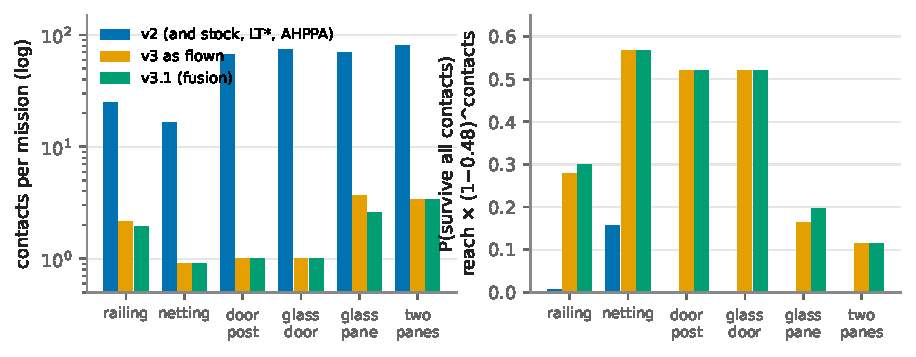
\includegraphics[width=1\linewidth,height=\textheight,keepaspectratio,alt={Fig.
3. Simulation under the bump model, 30 missions per scenario. Left:
contacts per mission (log scale); stock A*, Lazy Theta* and the shipped
portfolio behave like v2. Right: probability of surviving every contact
at 0.48 per contact.}]{figs/fig_bump.pdf}
\caption{Fig. 3. Simulation under the bump model, 30 missions per
scenario. Left: contacts per mission (log scale); stock A*, Lazy Theta*
and the shipped portfolio behave like v2. Right: probability of
surviving every contact at 0.48 per contact.}
\end{figure}

Every planner without contact memory bounced off the unmapped obstacle
until its time ran out: 41--42 \% of missions completed, all of them on
the railing and netting maps where the obstacle is eventually sensed,
with 17--80 contacts per mission. Contact memory completed every mission
with a median of one contact. Surface fusion mattered where contacts are
oblique and the obstacle is long: on the glass pane it reduced contacts
from 3.7 to 2.6 per mission and mission time from 50.7 to 42.5 s; over
all six scenarios it removed contacts in 15 missions and added them in 2
(paired Wilcoxon p = 0.0013); the worst mission fell from 8 contacts to
4, while one railing mission went from 1 contact to 3. On the two-pane
scenario neither variant improved on 3.4 contacts: the second pane is a
new surface, which no memory can anticipate.

\subsection{PX4 flights of v2, v3 and
v3.1}\label{px4-flights-of-v2-v3-and-v3.1}

We flew four batches in the \texttt{glass\_test} world: 20 flights of v2
and v3 before fusion existed (B20), 30 interleaved flights of v2, v3 and
v3.1 (B30), then 20 and 40 interleaved flights of v3 and v3.1 (B40,
B50). In each batch the order rotated every round and the goal
alternated between (8, 0) and (8, 2). A contact is counted from the pose
log (tilt ≥ 10° after at least 1 s below 5°, airborne) or from the
navigator's own impact detection, whichever is larger; every crash
counts as at least one contact.

\emph{Seven flights are excluded.} In B20 and B30 the test script
stopped waiting, and landed the drone, as soon as the navigator printed
``No 2.5D path found'' --- which the navigator also prints each time
contact memory relaxes. Every flight that relaxed its memory was
therefore landed early (after 50--86 s of simulated flight), with its
outcome unknown: four v3 and three v3.1 flights. We fixed the script (it
now waits only for the goal or a crash), raised the limit and disabled
PX4's battery failsafe for B40 and B50, and report the 103 remaining
flights in Table 3.

\begin{longtable}[]{@{}
  >{\raggedright\arraybackslash}p{(\linewidth - 6\tabcolsep) * \real{0.2000}}
  >{\raggedleft\arraybackslash}p{(\linewidth - 6\tabcolsep) * \real{0.2667}}
  >{\raggedleft\arraybackslash}p{(\linewidth - 6\tabcolsep) * \real{0.2667}}
  >{\raggedleft\arraybackslash}p{(\linewidth - 6\tabcolsep) * \real{0.2667}}@{}}
\caption{Table 3. PX4/Gazebo flights against the unseen pane, four
batches pooled, seven harness-cut flights excluded. Contacts per flight
is not a measure of quality: a crash ends the flight, so a planner that
survives contacts has more of them.}\tabularnewline
\toprule\noalign{}
\begin{minipage}[b]{\linewidth}\raggedright
\end{minipage} & \begin{minipage}[b]{\linewidth}\raggedleft
v2
\end{minipage} & \begin{minipage}[b]{\linewidth}\raggedleft
v3
\end{minipage} & \begin{minipage}[b]{\linewidth}\raggedleft
v3.1
\end{minipage} \\
\midrule\noalign{}
\endfirsthead
\toprule\noalign{}
\begin{minipage}[b]{\linewidth}\raggedright
\end{minipage} & \begin{minipage}[b]{\linewidth}\raggedleft
v2
\end{minipage} & \begin{minipage}[b]{\linewidth}\raggedleft
v3
\end{minipage} & \begin{minipage}[b]{\linewidth}\raggedleft
v3.1
\end{minipage} \\
\midrule\noalign{}
\endhead
\bottomrule\noalign{}
\endlastfoot
Valid flights & 20 & 46 & 37 \\
Reached the goal & 1 (5 \%) & 14 (30 \%) & 13 (35 \%) \\
Crashed & 19 (95 \%) & 32 (70 \%) & 19 (51 \%) \\
Gave up the goal & 0 & 0 & 5 \\
Survived the first contact & 5 (25 \%) & 34 (74 \%) & 33 (89 \%) \\
Crashes per contact & 0.68 & 0.30 & 0.25 \\
Contacts per flight & 1.40 & 2.28 & 2.08 \\
Reached, goal (8, 0) / (8, 2) & 1/10, 0/10 & 9/24, 5/22 & 10/19, 3/18 \\
Mean time to goal (s) & 74 & 104 & 88 \\
\end{longtable}

\begin{figure}
\centering
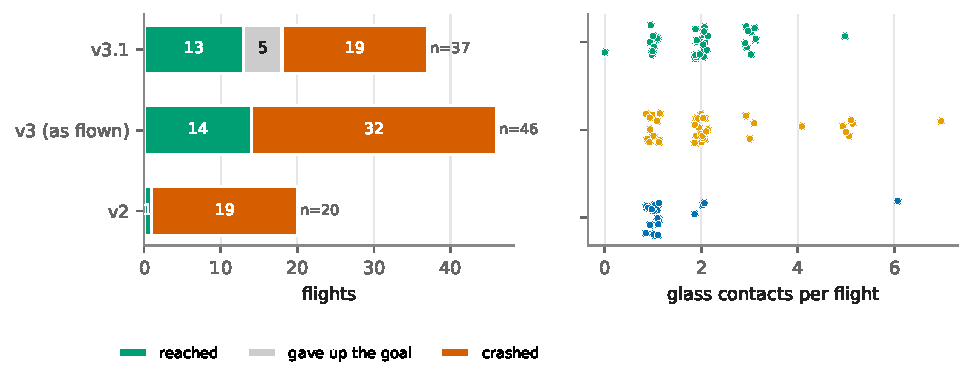
\includegraphics[width=1\linewidth,height=\textheight,keepaspectratio,alt={Fig.
4. PX4 flights. Left: outcome of every valid flight. Right: glass
contacts per flight (jittered).}]{figs/fig_px4.pdf}
\caption{Fig. 4. PX4 flights. Left: outcome of every valid flight.
Right: glass contacts per flight (jittered).}
\end{figure}

\textbf{Contact memory against v2.} Pooled over v3 and v3.1 (83
flights), contact memory crashed in 51 flights against 19 of 20 for v2
(Fisher p = 0.003) and reached the goal in 27 against 1 (p = 0.012). The
largest effect is not the memory but the reaction that comes with it. v2
has no impact detector: after a contact it keeps flying its plan,
re-approaches while still disturbed and loses control. v3 and v3.1
detect the contact, hold for the drone to steady and back off before
replanning. With that reaction 67 of 83 flights survived their first
contact, against 5 of 20 (p \textless{} 0.001), and the crash rate per
contact fell from 0.68 to 0.28. The bump-model simulation uses one crash
probability for all planners and therefore \emph{understates} the
benefit of contact memory.

\textbf{v3.1 against v3.} Fusion changes nothing until memory relaxes,
so we compare the relaxed flights of the 60 flown with the fixed script
(B40, B50). The eight v3 flights, relaxing to `dot', hit the pane 7, 5,
5, 5, 4, 3, 5 and 5 times (mean 4.9); the six v3.1 flights, relaxing to
`hull', hit it 3 times each (Mann-Whitney p = 0.002). Fusion therefore
does in flight what it does in simulation: it stops the drone returning
to the same pane. It did not raise the success rate. Five of the eight
relaxed v3 flights reached the goal against two of the six v3.1 flights
(p = 0.59), and over all 60 fixed-script flights v3.1 reached the goal
in 9 and crashed in 16, v3 in 11 and 19 (p = 0.78 and 0.60). At about
0.3 crashes per contact, two fewer contacts in the few flights that
relax is an effect these batches cannot resolve. Fig. 5 shows one flight
per variant.

\begin{figure}
\centering
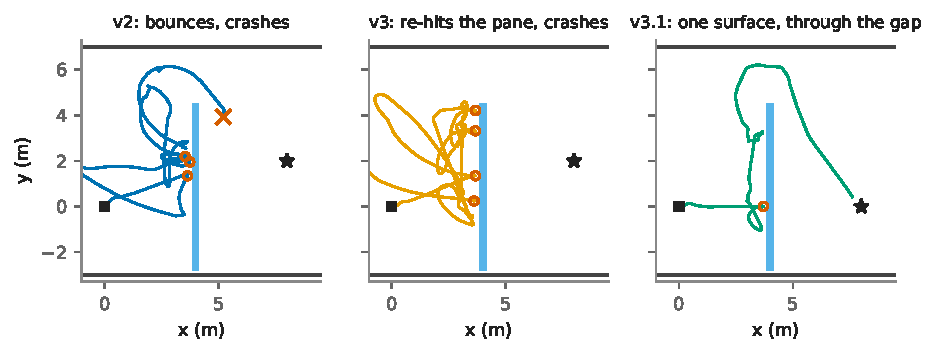
\includegraphics[width=1\linewidth,height=\textheight,keepaspectratio,alt={Fig.
5. One PX4 flight per variant, goal at the star (circles: contact
onsets; cross: crash). v2 (B20-v2-8) bounces off the pane and crashes;
v3 (B40-v3-10) relaxes its memory to single points and hits the same
pane five times before crashing; v3.1 (B30-v31-1) hits the pane, fuses
the contacts into one surface and goes round the
end.}]{figs/fig_traj.pdf}
\caption{Fig. 5. One PX4 flight per variant, goal at the star (circles:
contact onsets; cross: crash). v2 (B20-v2-8) bounces off the pane and
crashes; v3 (B40-v3-10) relaxes its memory to single points and hits the
same pane five times before crashing; v3.1 (B30-v31-1) hits the pane,
fuses the contacts into one surface and goes round the end.}
\end{figure}

\textbf{Failures that remain.} Most v3.1 crashes came at the first or
second contact, before memory can help. Five v3.1 flights, and no v3
flight, ended with the navigator giving up (p = 0.015): the map flagged
an obstacle on the path, no plan could be found from the drone's
position --- not even by the 2D fallback, which ignores contact memory
--- and the stock navigator dropped the goal. Fusion cannot cause this:
one of the five flights had no contact and the others one, and a single
barrier is never fused, so v3.1 planned exactly as v3 would. We have not
yet found the cause.

\section{Discussion and limitations}\label{discussion-and-limitations}

\emph{The first contact is not prevented.} Contact memory guarantees
nothing about the first contact with an obstacle the sensor cannot see;
with a 0.5 crash probability per contact, the best possible success rate
against an unseen pane is about 50 \%. Preventing the first contact
needs perception (glass detection \autocite{mei2020glass}) or an
airframe that tolerates contact \autocite{briod2014gimball}; contact
memory is complementary to both, and makes their residual failures less
likely to repeat.

\emph{Crash probability per contact is an estimate from one airframe in
one simulator, and it depends on the planner.} The simulator's 0.48 came
from the first 33 contacts at a cruise speed of about 0.3 m/s, with the
drone's altitude loss after contact as the dominant crash mechanism.
Over all valid flights it was 0.68 for v2, which presses on after a
contact, and 0.30 for the variants that hold and back off. Lower speeds,
prop guards or a different attitude controller would change it; the
ranking of planners in simulation does not depend on its value (Table 2,
last column) but the absolute success rates do.

\emph{The wall hypothesis can be wrong.} A 4 m barrier from a single
contact can seal a real passage; the relaxation ladder recovers, at the
cost of a re-contact in the worst case. In the simulated scenarios
relaxation was needed in 50 of 210 v3.1 missions (55 relaxations,
against 96 for v3, whose ladder lacks the hull level).

\emph{Fusion's benefit to outcomes is not confirmed in flight.} The
flights confirm the mechanism (fewer re-contacts after relaxation) but
not a higher success rate; relaxation happened in only 14 of 60
fixed-script flights.

\emph{The test harness mattered.} Seven flights were lost to a script
that treated a normal log message as the end of the flight. We found it
only by reading the logs of flights that appeared to time out; outcome
labels in batch flight tests should be checked against the trajectories.

\emph{Giving up is the navigator's default.} When no path exists from
the drone's cell, the navigator drops the goal. After a contact the
drone often hovers next to the obstacle, where this is most likely;
backing off further and retrying would turn these failures into further
attempts.

\emph{Simulation and SITL only.} All flights are software-in-the-loop;
real glass, real depth noise and real propeller strikes remain to be
tested.

\section{Conclusion}\label{conclusion}

A planner can only be as safe as its map. We found that an adaptive
portfolio of path planners does not beat its best member on indoor maps,
that a cheap smoothing step makes grid A* as short as any-angle
planning, and that the deadlocks an escape mode is built for come from
obstacles the map never holds. Contact memory --- writing what the drone
has \emph{touched} into every later plan, fusing contacts into surfaces
and relaxing them in steps --- turns repeated collisions into, in the
median, a single one. In PX4 flights the reaction to a contact mattered
as much as the memory: a drone that stops and backs off survives
contacts that a drone pressing on does not, and contact memory crashed
in 61 \% of flights where v2 crashed in 95 \%. Fusing contacts into
surfaces cut re-contacts in flight as in simulation; whether it also
raises the success rate needs more flights than we have.

\printbibliography[title=References]

\end{document}
